$subject$=Дополнительные главы \\ высшей математики
$date$=07.02.2025
$teacher$=Лекции Далевской О. П.

\section{1. Основные понятия}

\subsection{1.1. Комплексное число}

\Mem $\Complex = \{ (a, b) \ | \ a, b \in \Real\}$

Обозначение: $z = (a, b) = a + bi$, где $i = (0, -1) = \sqrt{-1}$

\underline{Основные операции}:

\begin{enumerate}
    \item $\RE z = a$ - вещественная часть, $\IM z = b$ - мнимая часть
    \item $z_1 + z_2 = (a_1, b_1) + (a_2, b_2) = (a_1 + a_2, b_1 + b_2) = (a_1 + a_2) + i(b_1 + b_2)$
    \item $z_1 \cdot z_2 = (a_1 + b_1 i) * (a_2 + b_2 i) = (a_1 a_2 - b_1 b_2) + i (a_1 b_2 + a_2 b_1)$
    \item $z^n = \rho^n (\cos n\varphi + i \sin n\varphi)$ - \textbf{формула Муавра}, где $\rho = |z|, \varphi = \arg z$
    \item $\sqrt[n]{z} = \sqrt[n]{\rho} \left(\cos \frac{\varphi + 2\pi k}{n} + i \sin \frac{\varphi + 2\pi k}{n}\right)$, где $\rho = |z|, \varphi = \arg z, k \in \Integer$
    \item При $n = 2$ $\sqrt{z} = \sqrt{a + bi} = \pm (c + di)$, 
        где $c = \sqrt{\frac{a + \sqrt{a^2 + b^2}}{2}}, d = \operatorname{sign}(b) \sqrt{\frac{-a + \sqrt{a^2 + b^2}}{2}}$
\end{enumerate}

\begin{minipage}{\textwidth}
    % https://www.geogebra.org/calculator/xjg67fnv

    \begin{wrapfigure}{r}{0pt}
        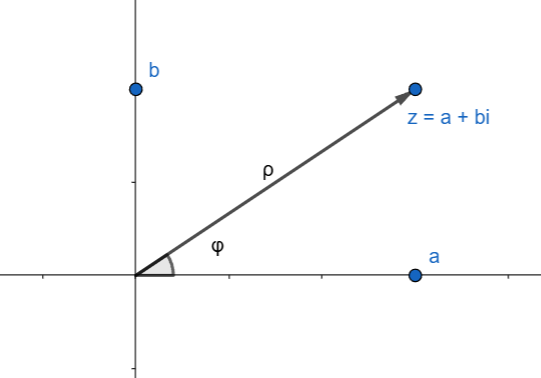
\includegraphics[width=7cm]{addchapters2/images/addchapters2_2025_02_07_6}
    \end{wrapfigure}

    Тригонометрическая форма:

    $z = a + bi = \rho (\cos \varphi + i \sin \varphi)$, где $\rho = |z| = \sqrt{a^2 + b^2}, \varphi = \arg z \in [0; 2\pi)$

    $\Arg z = \arg z + 2\pi k, k \in \Integer$

    По формуле Эйлера $z = \rho (\cos \varphi + i \sin \varphi) = \rho e^{i \varphi}$
\end{minipage}

\subsection{1.2. Комплексная плоскость}

\Def Окрестность точки $z_0 \in \Complex$ определяется как $U_\delta (z_0) = \{z \in \Complex \ \Big| \ |z - z_0| < \delta\}$

Тогда $\overset{\circ}{U}_\delta (z_0) = U_\delta (z_0) \setminus \{ z_0 \}$ - выколотая окрестность

\Def Для данной множества точек $A$ точка $z_0$ считается

\begin{itemize}
    \item внутренней, если для любого $\delta$ $U_\delta (z_0) \subset A$
    \item граничной, если для любого $\delta$ $\exists z \in U_\delta (z_0) \Big| z \in A$ и $\exists z \in U_\delta (z_0) \Big| z \notin A$
\end{itemize}

\Def Открытое множество состоит только из внутренних точек

\Defs Закрытое множество содержит все свои граничные точки

\Defs Границой $\Gamma_D$ (иногда обозн. $\delta D$) для множества $D$ называют множество всех граничных точек $D$

\Defs Если любые две точки множества можно соединить ломаной линией конечной длины, то множество считается связным

\Defs Множество $D \subset \Complex$ называется областью, если $D$ - открытая и связная

\Defs Кривая $l \subset \Complex$ считается непрерывной, если $l = \{z \in \Complex \ | \ z = \varphi(t) + i \psi(t), t \in \Real\}$, где $\varphi(t), \psi(t)$ - непрерывные функции

\Notas Если $\varphi(t)$ и $\psi(t)$ дифференцируемы и их производные непрерывные, то кривая $l$ гладкая

\Defs Непрерывная замкнутая (то есть начальная и конечная точки совпадают) без самопересечений кривая называется контуром

\Notas Односвязную область можно стянуть в точку

% https://www.geogebra.org/calculator/nhbjhbag

\begin{multicols}{2}
    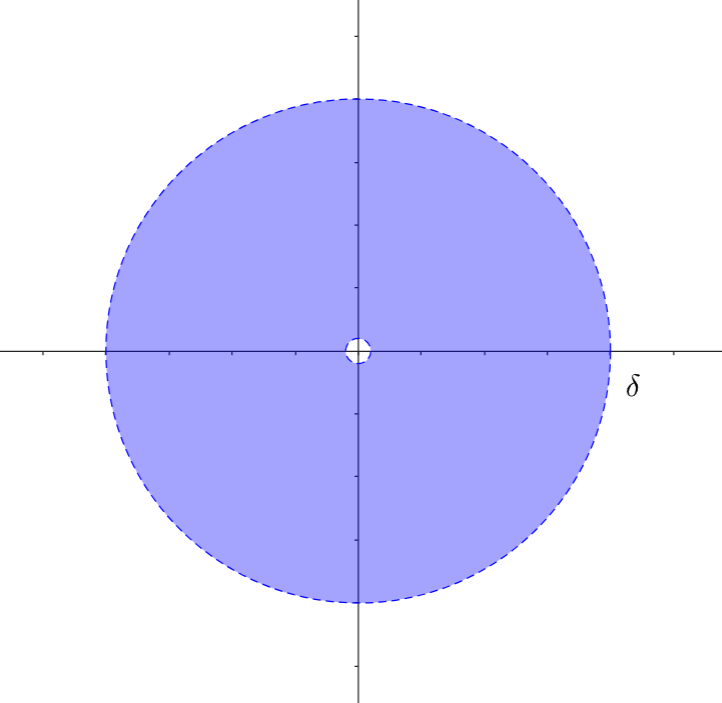
\includegraphics[width=0.4\textwidth]{addchapters2/images/addchapters2_2025_02_07_1}

    \ExNs{1} $D = \{z \in \Complex \ \Big| \ 0 < |z| < \delta\}$ - область связаная, но не односвязная, ее нельзя стянуть из-за дырки

    \mediumvspace

    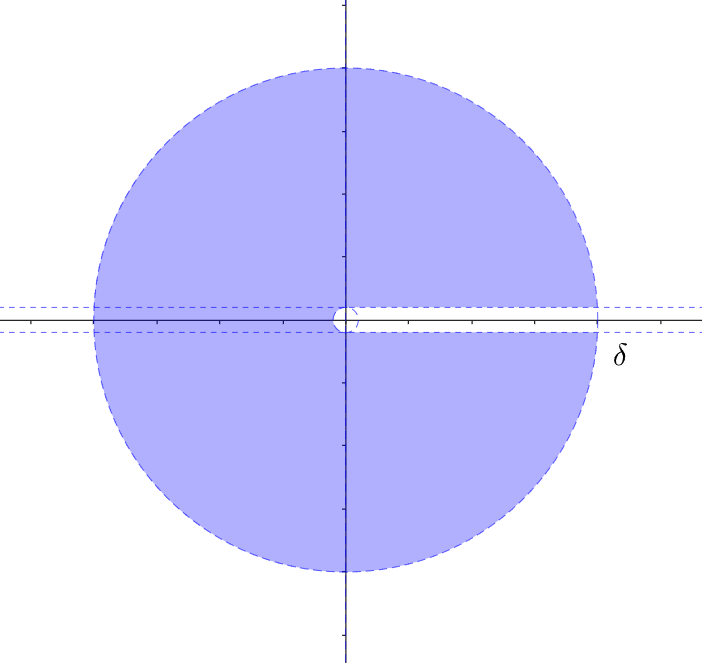
\includegraphics[width=0.4\textwidth]{addchapters2/images/addchapters2_2025_02_07_2}

    \ExN{2} $D = \{z \in \Complex \ \Big| \ 0 < |z| < \delta, \arg z \neq 0\}$ - область связная и односвязная
\end{multicols}

\begin{multicols}{2}
    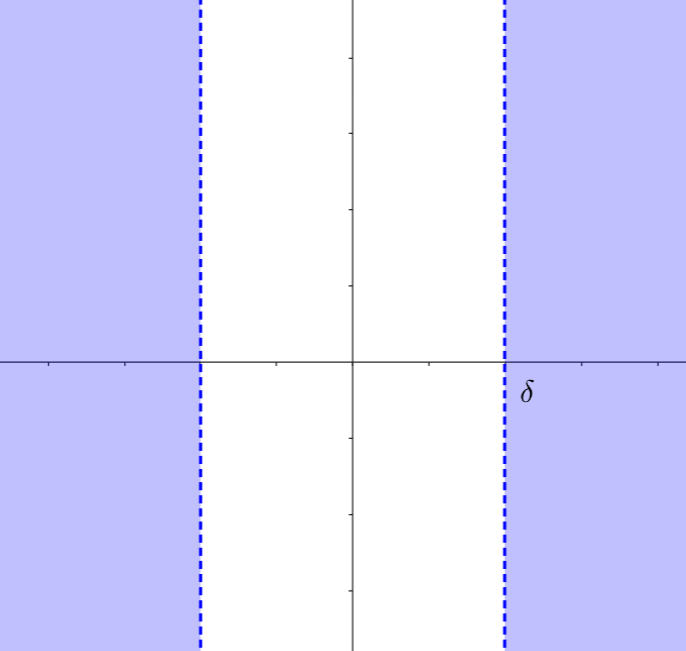
\includegraphics[width=0.4\textwidth]{addchapters2/images/addchapters2_2025_02_07_3}

    \ExN{3} $D = \{z \in \Complex \ \Big| \ |\RE z| < \delta\}$ - несвязная область

    \mediumvspace

    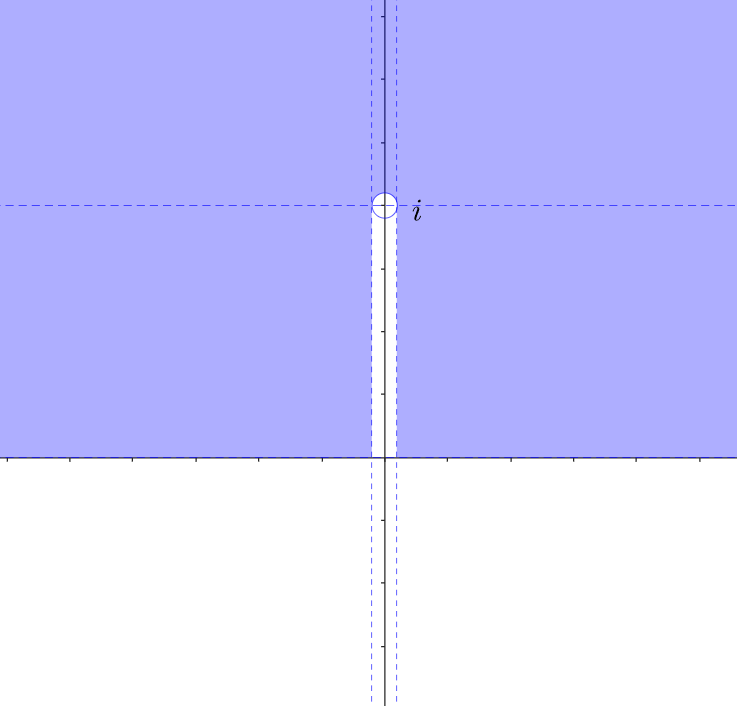
\includegraphics[width=0.4\textwidth]{addchapters2/images/addchapters2_2025_02_07_4}

    \ExN{4} $D = \{z \in \Complex \ \Big| \ \IM z \geq 0, z \notin [0, i]\}$ - здесь под $[0, i]$ подразумевается линейный отрезок на оси
\end{multicols}

\Nota Дальше все рассматриваемые $\Gamma_D$ будут состоять из кусочногладких и изолированных кривых

\subsection{1.3. Предел}

\Mem Последовательность $\{z_n\} = z_1, z_2, z_3, \dots, z_n, \dots$

\Def Пределом $\{z_n\}$ называют число $z$ такое, что

$\forall \varepsilon > 0 \ \exists \underset{n_0 = n_0(\varepsilon)}{n_0 = \Natural} \ \Big| \ \forall n > n_0 \ |z_n - z| < \varepsilon$

Обозначается $\lim_{n \to \infty} z_n = z$

\Nota $\{z_n\}$ можно представить как ${x_n + i y_n}$, то есть двумя $\Real$-последовательностями

\begin{MyTheorem}
    \Ths $\exists \lim_{n \to \infty} z_n = \underset{x, y \in \Real}{x + i y} \Longleftrightarrow $
    \begin{tabular}{l} $\exists \lim_{n \to \infty} x_n = \lim_{n \to \infty} \RE z_n = x$ \\ $\exists \lim_{n \to \infty} y_n = \lim_{n \to \infty} \IM z_n = y$ \end{tabular}
\end{MyTheorem}

\begin{MyProof}
    \fbox{$\Longleftarrow$} $\forall \varepsilon > 0 \ \exists \underset{n_0 = \max (n_{0x}, n_{0y})}{n_0 \in \Natural} \ \Big| \ \forall n > n_0 \begin{tabular}{l} |x_n - x| < \frac{\varepsilon}{2} \\ |y_n - y| < \frac{\varepsilon}{2} \end{tabular}$
    
    $|z_n - z| = |(x_n - x) + i(y_n - y)| \leq |x_n - x| + |y_n - y| < \frac{\varepsilon}{2} + \frac{\varepsilon}{2}$

    То есть $\forall \varepsilon > 0 \dots |z_n - z| < \varepsilon$

    \fbox{$\Longrightarrow$} $\forall \varepsilon > 0 \ |z_n - z| = |(x_n - x) + i(y_n - y)| < \varepsilon \Longrightarrow 
    \begin{cases}
        |x_n - x| \leq |(x_n - x) + i(y_n - y)| < \varepsilon \\
        |y_n - y| \leq |(x_n - x) + i(y_n - y)| < \varepsilon \\
    \end{cases} \Longrightarrow \exists \lim_{n \to \infty} x_n = x$ и $\exists \lim_{n \to \infty} y_n = y$

\end{MyProof}

\Nota Для комплексных чисел работают теоремы для пределов (сумма пределов, произведение пределов и т.д.), критерий Коши и другие

\Def $\lim_{n \to \infty} z_n = \infty \Longleftrightarrow \forall \varepsilon > 0 \ \exists \underset{n_0 = n_0(\varepsilon)}{n_0 \in \Natural} \ \Big| \ n > n_0 \ |z| > \varepsilon$

\Defs Точка $z$, определенная как предел, равный $\infty$, называется бесконечно удаленной. Но существует множество последовательностей, чьи пределы удаляются на бесконечность разными путями на плоскости

\Def Стереографическая проекция (сфера Римана)

% https://www.geogebra.org/calculator/kjesw2gx

\begin{center}
    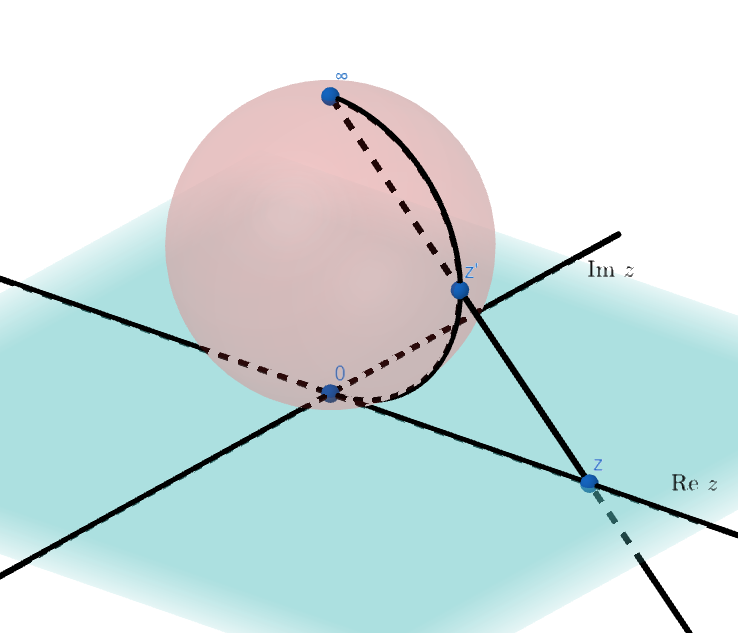
\includegraphics[width=0.55\textwidth]{addchapters2/images/addchapters2_2025_02_07_5}
\end{center}

Поместим сферу на комплексную плоскость и сделаем биекцию точек плоскости на точки сферы: проведем из верхней точки сферы лучи вниз на плоскость, и точка, где луч пересекает сфера,
будет считаться отображением для данной точки. Заметим, что в этом случае бесконечно удаленные точки будут отображаться в верхнюю точку сферы

\Def $\Complex \cup \{\infty\} = \overline{\Complex}$ - расширенная комплексная плоскость

Однако $z + \infty$ не определена, $\infty + \infty$ не определена. 
Но $\infty = \lim_{n \to \infty} \frac{1}{z_n}$ при $z_n \underset{n \to \infty}{\longrightarrow} 0$; $\infty = \infty \cdot \lim_{n \to \infty} z_n$ при $z_n \longrightarrow z$

Записью $[-\infty; +\infty]$ обозначается ось $\overline{\Real}$; 

\qquad\qquad $[-i\infty; +i\infty]$ - мнимая расширенная ось

Путь $x \pm i \infty$ при фикс. $x$ - вертикальная прямая; 

\qquad\qquad $iy \pm \infty$ - горизонтальная прямая; 

\qquad\qquad $e^{i\varphi} \cdot \infty$ - прямая, проходящая через начало координат


